\documentclass[a4paper,11pt,twocolumn]{article}
\usepackage{lingmacros}
\usepackage{blindtext}
\usepackage{tree-dvips}
\usepackage{amsmath}
\usepackage{multicol}
\usepackage{mathtools}
\usepackage{hyperref}
\usepackage{graphicx}
\usepackage{amssymb}
\usepackage[table]{xcolor}
\graphicspath{ {./Latex/} }
%\usepackage{wrapfig}

\begin{document}

\title{Solving differential equations using neural networks}
\date{2019\\ December}
\author{Eirik Nordgård\\ Geophysical Institute,\ University of Oslo}


\twocolumn[
\begin{@twocolumnfalse}
\maketitle
\begin{abstract}
In this paper a neural network is used for solving the diffusion equation, comparing the performance with a traditional finite difference approach using a Forward Euler scheme. Using the finite difference approach the resulting MSE ranges from order $10^{-4}$ to $10^{-6}$ with spatial steps $10^{-1}$ and $10^{-2}$ respectively. Results obtained by the neural network gives MSE on the order of $10^{-3}$ for spatial steps $10^{-1}$ and $10^{-2}$, which indicates that you can indeed solve the diffusion equation using a neural network. Despite providing low MSE, the neural network is slower compared to the finite difference approach.  
\
SOMETHING ON THE EIGENVALUES WHEN FOUND 

\end{abstract}

All material for this project may be found on 
\url{https://github.com/eirikngard/FYS-STK4155/tree/master/Project_3}

\end{@twocolumnfalse}
]
\
\section{Introduction}

Solving differential equations (DE's) is an important and central problem in physics, meteorology and many other fields. Doing so efficiently and accurately is therefore of great interest, and various algorithms have been used to sole this problem. Complex DE's typically require high order algorithms while simple DE's can be solved using first or second order algorithms such as Forward Euler Scheme. Time and computer power consumption is the main problem solving DE's. A coupled model computing several equations for thousands or millions of grid-boxes may suffer badly from a poor DE solving algorithm, both in terms of accuracy and time consumption.  
Intro on the field of differential equations and solving them. How to use a NN for solving a problem like this. The paper by Lagaris et. al. (1998)\cite{lagaris} is one of many that suggests solving DE's can be done with high precision using Neural Networks (NN's). However, the computational cost may be quite large. 
The question of interest regarding the use of NN's is whether they have the ability to outperform traditional algorithms in speed and efficiency. In this project this will be investigated comparing the Forward Euler approach with the Neural Network approach. Furthermore, following the approach in the paper by \cite{yi} et. al. (year), the NN will be used to compute extrema eigenvectors and corresponding eigenvalues. In this project the Diffusion Equation will be solved. Physically this equation can for example represent the temperature gradient through a rod, describing how the temperature decays along the rod with time.  
\\
\\
In section 2 all theory and background information and ideas will be presented, including the metrics used to evaluate the results. Section 3 describes how the algorithms are built and what they produce. In section 4 the methods used solving the diffusion equation will be compared and main findings will be presented, and section 5 provides a discussion of pros and cons of the respective methods. Finally, section 6 provides a conclusion and suggestions for future work.   
\
\section{Theory}

\subsection{The general problem}

The problem to be solved is the simple diffusion equation
\begin{equation}
\frac{\partial u(x,t)}{\partial t}=\frac{\partial{^2}u(x,t)}{\partial x^2} \quad t>0 \quad x\in [0,L].
	\label{eq:diff}
\end{equation}
Another way to write this problem is $u_{xx} = u_t$. Initial conditions is necessary. Using $L=1$, the initial condition at $t=0$ is given by
\begin{equation}
    u(x,0) = \sin(\pi x)
    \label{eq:incond}.
\end{equation}
Furthermore, Dirichlet boundary conditions are also used, given by
\begin{equation*}
    u(0,t) = u(L,t) = 0 \quad t \geq 0.
\end{equation*}

As an example, this differential equation and its initial and boundary conditions could represent the temperature of a heated rod. As time progress the heat is transported through the rod while the temperature decreases along the way.


\subsection{Exact solution of the diffusion equation}
To investigate how the solutions to the partial differential equation performs it is necessary to compare them with some benchmark solution. The exact solution serves this purpose, and it will be calculated in this section. 
Through separation of variables, the exact solution can be expressed as
\begin{equation}
u(x,t) = X(x)T(t)
\label{eq:separated}
\end{equation}
Differentiating this according to \eqref{eq:diff} and moving some terms, we get
\begin{equation}
\frac{X''(x)}{X(x)} = \frac{T'(t)}{T(t)}
\label{eq:part}
\end{equation}
As the to sides of \eqref{eq:part} are not dependant on the same variables, they must both be equal to a constant. For convenience the constant is chosen to be $-\omega ^2$. This gives the two equations.
\begin{equation}
\begin{split}
X''(x) &= -\omega ^2 X(x) \\
T'(t) &= -\omega^2 T(t)
\end{split}
\label{eq:xt}
\end{equation}
Now the solution $X$ can appear in three possible ways given by the characteristic equation. In order to satisfy the initial condition \eqref{eq:incond}, $X(x)$ must be on the form
\begin{equation*}
X(x) = B\sin(\omega x) + C\cos(\omega x)
\end{equation*}
The initial condition then rules $C=0, \omega = \pi$. For $T(t)$ in \eqref{eq:xt} the solution is on the form
\begin{equation*}
T(t) = Ae^{-\omega^2t}
\end{equation*}
As we know $\omega =\pi$, the solution is then:
\begin{equation*}
u(x,t) = X(x)T(t) = Ae^{-\pi^2 t}B\sin(\pi x)
\end{equation*}
Finally, from the initial condition, we know that $A\cdot B = 1$, hence the exact solution denoted \textit{exact} must be
\begin{equation}
u_{exact}(x,t) = e^{-\pi^2 t}\sin(\pi x)
\label{eq:exact}
\end{equation}

\subsection{Solution using explicit Euler scheme}

Now it is desired to solve the equation with a Euler scheme. To make this possible, eq. \eqref{eq:diff} must be discretized in both time and space. As time is only used in first order derivative, we will use the explicit Forward Euler Scheme, which gives an error proportional to $\Delta t$ \cite{boyces}. This scheme is given as
\begin{equation}
  {u(x,t)}{t} \approx \frac{u(x,t+\Delta t) - u(x,t)}{\Delta t}
    \label{eq:foreward}
\end{equation}
For the spatial discretization a centred difference is used, which has an error proportional to $\Delta x^2$ \cite{boyces}, given by
\begin{equation}
 {u(x,t)}{x} = \frac{u(x+\Delta x,t) - 2u(x,t) + u(x-\Delta x,t)}{\Delta x^2}
    \label{eq:centerd}
\end{equation}
on a discrete time and space grid, $u(x,t) = u(x_i,t_n)$, $t+\Delta t_n = t_{n+1}$ and so on.
Simplifying this notation yields $u_i^n = u(x_i,t_n)$. On a discrete form eq. \eqref{eq:diff} is then 
\begin{equation}
\begin{split}
    u_{xx} &= u_t \\
    [u_{xx}]_i^n &= [u_t]_i^n \\
    \frac{u_{i+1}^n - 2u_i^n + u_{i-1}^n}{\Delta x^2} &= \frac{u_i^{n+1}-u_i^n}{\Delta t}
\end{split}
\end{equation}
Solving this for $u_i^{n+1}$ provides the solution $u$ to \eqref{eq:diff} for each spatial point $i$:
\begin{equation}
    u_i^{n+1} = \frac{\Delta t}{\Delta x^2}(u_{i+1}^n - 2u_i^n + u_{i-1}^n)  + u_i^n
    \label{eq:euler}
\end{equation}
\eqref{eq:euler} is stable for the following grid resolutions:
\begin{equation*}
    \frac{\Delta t}{\Delta x^2} \leq \frac{1}{2}
\end{equation*}


\subsection{Solution using a Neural Network}
Solving the PDE can also be done using a neural network. For more in depth information on neural networks and how they work, see git repository Project2 \cite{gitrepo}. In this project the neural network functionality within \textit{TensorFlow} for python3 is used, as this is stable, fast and simple to use compared to building a neural network from scratch. 

In order to solve PDEs with a neural network, we approximate the true function $u$ with a trial function $\Theta (x,t)$. Thus the aim is to calculate $\Theta$ as close to the true function $u$ as possible \cite{lagaris}. When aiming to solve Eq. \eqref{eq:diff}, the corresponding equation for the trial function is
\begin{equation*}
   {\Theta(x,t)}{x} = {\Theta(x,t)}{t} \quad t>0 \quad x\in [0,L]
\end{equation*}
The residual of this approximation is then
\begin{equation}
    E = {\Theta(x,t)}{x} - {\Theta(x,t)}{t}
    \label{eq:error}
\end{equation}
The cost function to be minimized by the Neural Network is the sum of $E$, evaluated at each point in the space and time grid. This equivalent to minimizing the mean squared error. The neural network iterates a given number of times. For each iteration the trial function is updated based on the networks previous calculated trial function. Choosing the correct "form" of the trial function is important to restrain the residual, and this "form" is based on the order of the PDE and its initial condition. To satisfy both the initial condition and the Dirichlet condition of Eq. (\ref{eq:diff}), the following form is chosen:
\begin{equation}
    \Theta (x,t) = (1-t)I(x) + x(1-x)tN(x,t,p),
    \label{eq:trial}
\end{equation}
where $I(x)$ is the initial condition, $N(x,t,p)$ is the output from the neural network and $p$ is the weights and biases of the network. 

Ideally the process should work accordingly: For each iteration in the network, the partial derivatives of $\Theta$ is calculated according to the new state of the network $N(x, t, p)$, updating the cost along the way. As the cost is minimized, the error term $E$ gets closer to zero, and the trial function $\Theta (x,t)$ approaches the true solution of the PDE. In theory the cost can practically reach zero if the number of iterations is big enough, but since it is of small interest to run infinite iteration a \textit{minimum cost value} is chosen to $10^{-3}$. Learning rate, the structure of the neural network in terms of the number of hidden layers and the number of nodes in each layer is also important in minimizing the cost. 

\subsection{Computing eigenpairs with Neural Networks}

It is also desired to solve another problem using the neural network, namely computing the eigenvectors $\Lambda$ and corresponding eigenvalues $\lambda$ of a symmetric matrix $A$.

Yi et. al. (2004) \cite{yi} provides a neat way to compute $\Lambda_{max}$ and $\lambda_{max}$ is provided. This computation is done by solving the ordinary differential equation
\begin{equation}
	\frac{d\Lambda(t)}{dt} = -\Lambda(t) + f(\Lambda(t)), \quad t\geq 0
	\label{eq:eigen2}
\end{equation}
 where $\Lambda = [\Lambda,\Lambda,\ldots,\Lambda_n]^T$ and $f(\Lambda)$ is given as
 %\begin{equation}
 %f(\Lambda) = \left v^Tv A + \left(1-\v^T Av\right)I\right]v
 %	\label{eq:f}
%\end{equation}
Here it is an equation for f from YI.
Here, $I$ is the $n\times n$ identity matrix. 

According to \cite{yi}, when $t\rightarrow \infty$, any random non-zero initial $\Lambda$, will approach $\Lambda_{max}$ if it is not orthogonal to $\Lambda_{max}$. The corresponding eigenvalue $\lambda_{max}$, is computed by the equation 

\begin{equation}
	\lambda = \frac{v^TAv}{v^Tv}
	\label{eq:eigenvalue}
\end{equation}
In \eqref{eq:eigenvalue} A is a symmetric matrix given by

\begin{equation}
	A = \frac{Q^T+Q }{2}
	\label{eq:symmetric}
\end{equation}
where $Q$ is a random, real matrix. 

After finding the largest eigenvalue $\lambda_{max}$, the smallest eigenvalue $\lambda_{min}$ corresponding to the eigenvector $\Lambda_{min}$ is easily found by substituting $A$ with $-A$ in Eq. (\ref{eq:symmetric})\cite{yi}.
\\

To solve eq. (\eqref{eq:eigen2}) with a neural network a trial solution is proposed. Since $v \in \mathbb{R}^n$, we choose a trial function $\Psi(x,t)$ dependent both on position $x$ and time $t$, so that for each time step, the approximated eigenvector is given as $[v(1,t), v(2,t), \ldots, v(n,t)]^T$. Eq. \ref{eq:eigen2} can then be rewritten as
\begin{equation}\label{eq:trial_eigen}
	\frac{\partial \Psi(x,t)}{\partial t} = -\Psi(x,t) + f(\Psi(x,t))
\end{equation}
with $t \geq 0$ and $x=1,2,\ldots,n$. We defined the trial function as 
\begin{equation*}
	 \Psi(x,t) = v_0 + tN(x,t,p)
\end{equation*}
where $v_0$ is the initial $v$, chosen at random.   
The error is then the difference between the two hand sides of Eq. (\ref{eq:trial_eigen}). 

\subsection{Metrics used to evaluated solutions}

The main metric used to evaluate the performance of the neural network compared to the analytic scheme is the Mean Squared Error (MSE). As the name suggests, this metric quantifies the mean of the squares of the error between the prediction $\hat{x}_i$ and the observed value $x_i$. Thus, 

\begin{equation*}
MSE = \frac{1}{n}\sum_{i=1}^n (x_i - \hat{x}_i)^2
\end{equation*}

where $n$ is the number of samples. MSE value of 0 would prediction of the observed value, thus the closer to zero the better prediction.  
 

\section{Method - implementation of algorithms}
Solving the problem with the Forward Euler Scheme is done iterating in time and space over equation \eqref{eq:euler}, returning $u$ and $x$ values for a given initial function and total time $T$. Thereafter the solutions are plotted and the mean squared error from the exact solution is calculated. 
\\
The neural network is build using functionalities of \textit{tensorflow}. It solved the diffusion equation using a given number of layers, neurons, total time and learning rate. A cost function is calculated based on a trial solution, which is then minimized. The network iterates until a given threshold cost value is reached, then return $u$ and $x$. Thereafter the solutions are plotted and the mean squared error from the exact solution is calculated.  
\\
Computing the eigenpairs is done using the approach described in section 2.5. Functions defining the function $f$ and the eigenvalues are defined and calculated using the symmetric matrix $A$. Then the neural network is designed similarly to the one described above, now returning eigenvectors $v_{dnn}$, a time vector $t$ and number of completed iterations $i$. The eigenvectors produced by the network is then used to calculate eigenvalues, which is then plotted with time to verify convergence. Also, \textit{numpy.linalg} is used to calculate reference eigenpairs. 

\section{Results}

In Figure \ref{euler} the solution of the diffusion equation by the Forward Euler Scheme is displayed. Blue lines are solution after 0.02 seconds, while red lines are solutions after 0.2 seconds. Inspecting Figure \ref{euler} immediately reveals that the analytic solution of the equation is very good, and that smaller spacial steps provides a solution closest to the exact solution. Also, we observe that the solution for the spatial step $\delta x = 0.1$ is closer to the exact solution at $t = 0.2$ than at $t = 0.02$. For both moments in time the solution for spatial step $\delta x = 0.01$ is very hard to distinguish from the exact solution, meaning it is a very good approximation. 


\begin{figure}[h]
	\centering 
	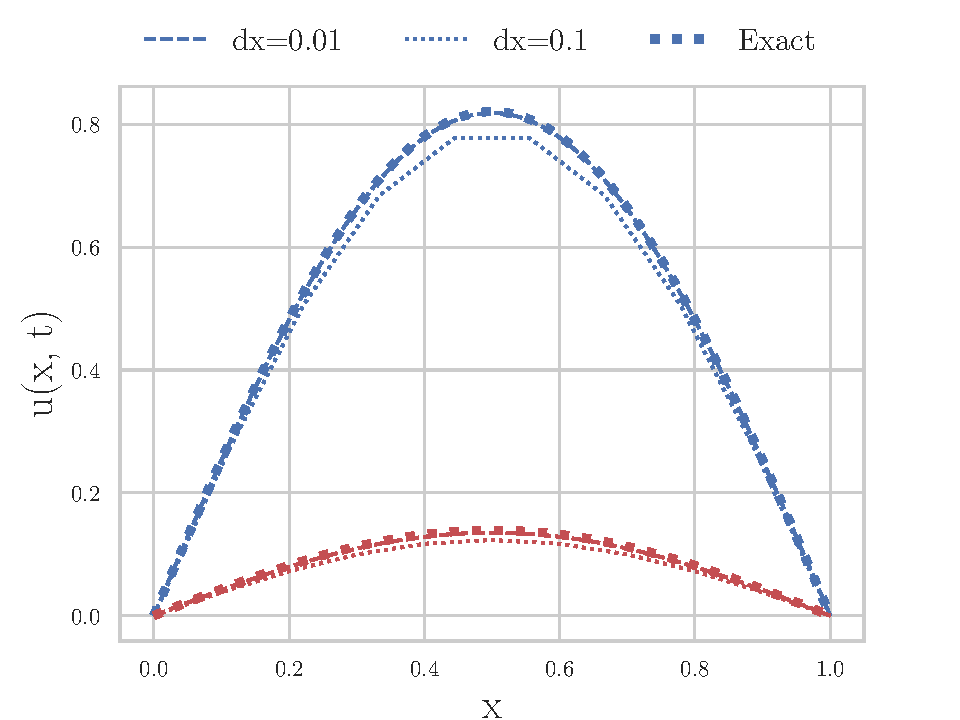
\includegraphics[width=0.5\textwidth]{figures/euler}
	\caption{Solution of the diffusion equation using Forward Euler Scheme. Solutions for $\delta x = 0.1$ and $\delta x = 0.1$ are displayed with the exact solution. Blue lines are solutions after 0.02 seconds. Red lines are solution after 0.2 seconds.}
	\label{euler}
\end{figure}

In Fig.\ref{fig:nn} the diffusion equation is solved using a neural network with Nt = 10, Nx = 100 and two hidden layers with 20 neurons each. The learning rate was set to $10^{-3}$ and the number of iterations was set to $10^3$. 

\begin{figure}[h]
	\centering 
	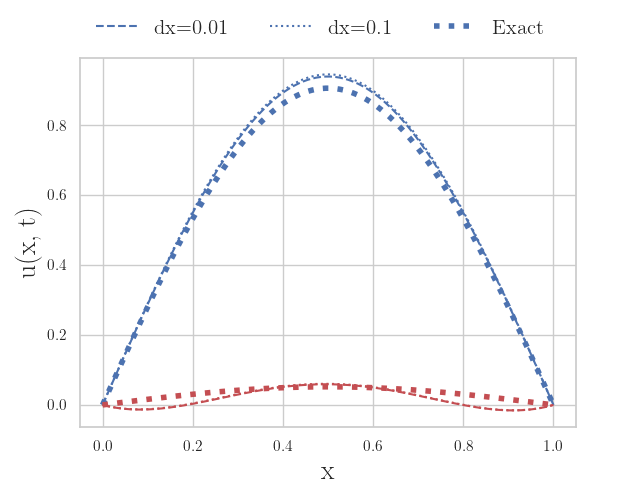
\includegraphics[width=0.5\textwidth]{figures/NN}
	\caption{Solution of the diffusion equation using a Neural Network. Solutions for $\delta x = 0.1$ and $\delta x = 0.1$ are displayed with the exact solution. Blue lines are solutions after 0.02 seconds. Red lines are solution after 0.2 seconds.}
	\label{fig:nn}
\end{figure}

A 3D visualization of the diffusion equation solved by the neural network can be found in Figure \ref{3dnn}.

\begin{figure}[h]
	\centering 
	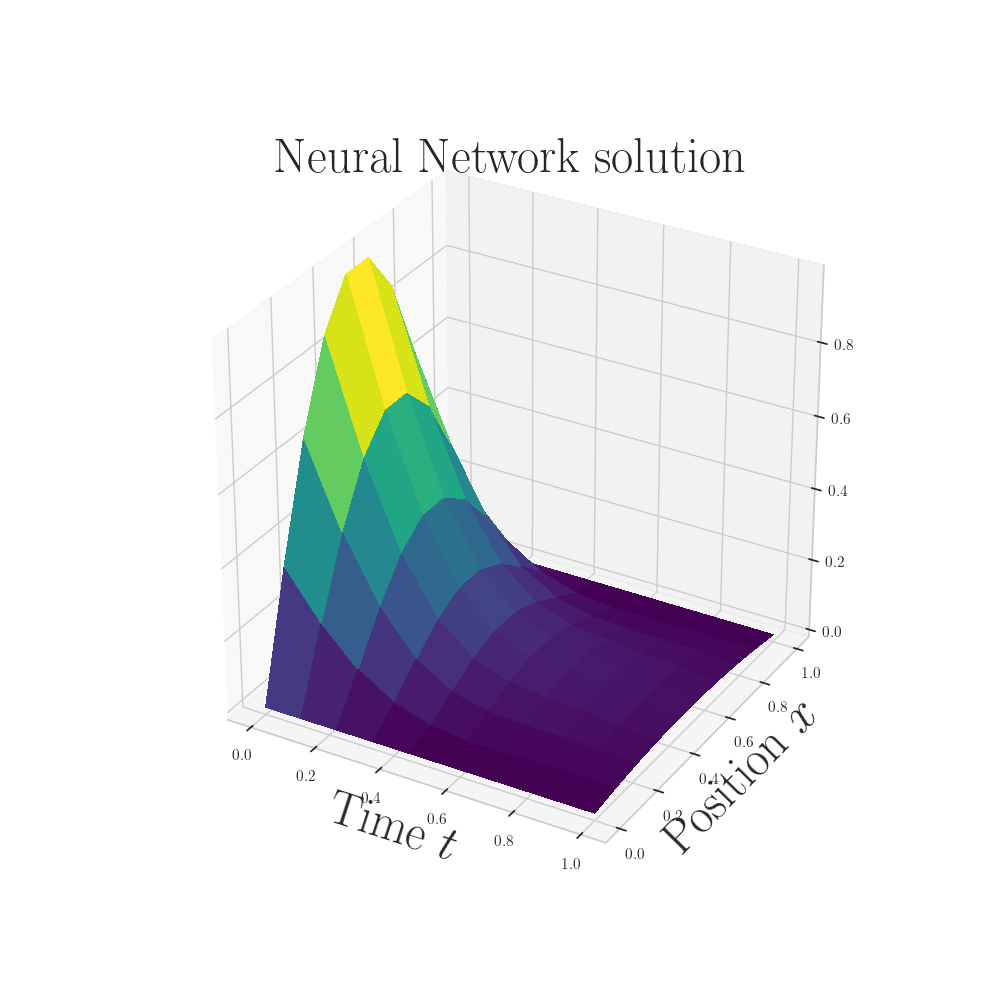
\includegraphics[width=0.5\textwidth]{figures/dnn}
	\caption{Solution of the diffusion equation using a Neural Network. Nt = 10, Nx = 100 and $10^3$ iterations was done. }
	\label{3dnn}
\end{figure}

Running the Euler Scheme we get the following MSE scores:

\begin{figure}[h]
	\centering 
	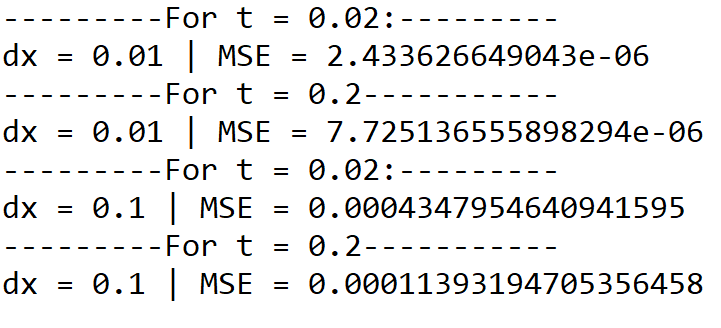
\includegraphics[width=0.5\textwidth]{figures/euler_mse}
	\caption{MSE from the Euler solution at $t = 0.2s$ and $t = 0.02s$ with different spacial steps.}
	\label{eulermse}
\end{figure}

Running the Neural Network we get the following MSE scores:

\begin{figure}[h]
	\centering 
	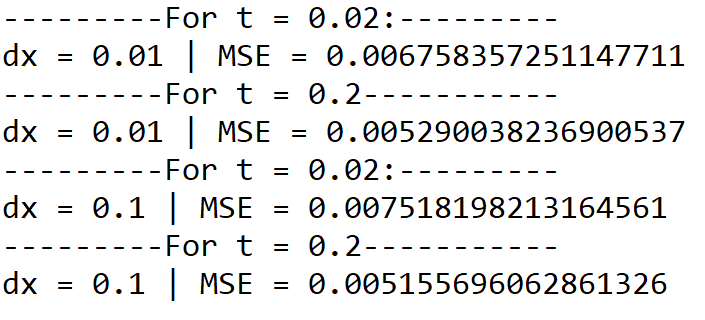
\includegraphics[width=0.5\textwidth]{figures/nnn_mse}
	\caption{MSE from the neural network solution at $t = 0.2s$ and $t = 0.02s$ with different spacial steps.}
	\label{nnmse}
\end{figure}

The neural network is very slow in solving the differential equation compared to the analytical solution.
\subsection{Eigenvectors and eigenvalues}

Using the approach provided by Yi et. al (2004) \cite{yi}, the neural network produced eigenvalues displayed in Figure (\ref{fig:eigenval1} and Figure (\ref{fig:eigenval2}).

\begin{figure}[h]
	\centering 
	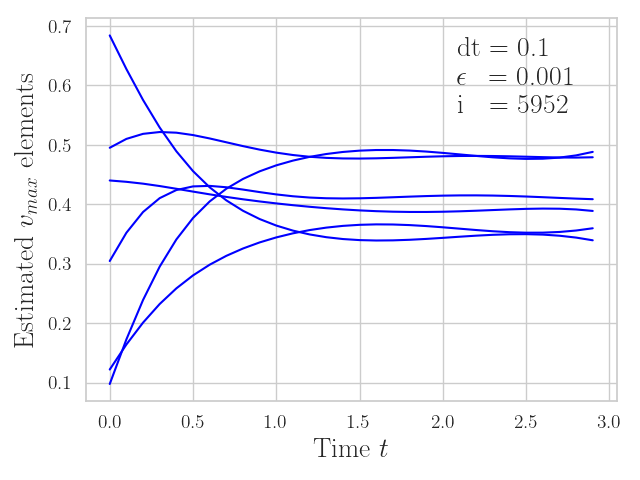
\includegraphics[width=0.5\textwidth]{figures/eigenvalues1}
	\caption{Time evolution of $v_{max}$.}
	\label{fig:eigenval1}
\end{figure}

\begin{figure}[h]
	\centering 
	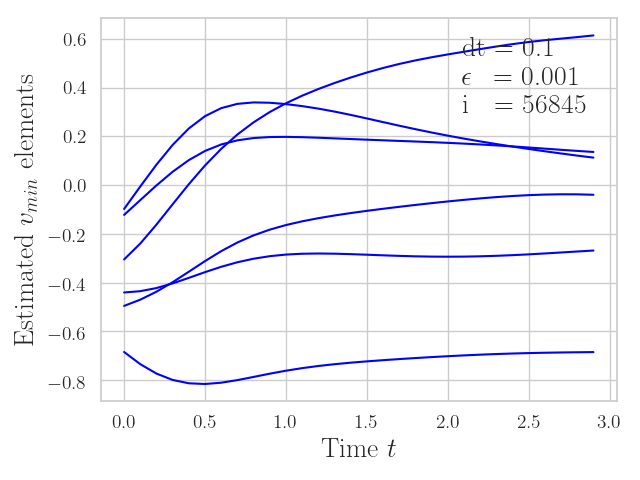
\includegraphics[width=0.5\textwidth]{figures/eigenvalues2}
	\caption{Time evolution of $v_{min}$.}
	\label{fig:eigenval2}
\end{figure}

The target cost value was set to $10^{-3}$ because the algorithm was very slow for any lower values. As displayed in Figure (\ref{fig:eigenval2}), the required number of iteraations to calculate the $v_{min}$ eigenvalue was 56845. It is also evident from Figure (\ref{fig:eigenval1}) and Figure (\ref{fig:eigenval2}) that the network can in fact calculate the eigenvalues, as almost all of the seem to converge at some value with time. 
\section{Discussion}
Letting the finite difference approach serve as a benchmark, the MSE is on the order of $10^3$ for $\delta x = 0.01$ and $10^1$ for $\delta x = 0.1$ lower than for the neural network. This is partly because the target MSE value for the neural network was chosen to $10^{-3}$ due to an issue with time consumption. Allowing the network to iterate to lower MSE values was possible, but required lots of time to complete, making the code close to useless. Depending on what model the neural network could have been used in, the MSE of the neural network is still quite good. However, in a complex model the Euler solution would be preferred over the neural network. Keeping the calculation error as small as possible is often crucial for obtaining good result over time. Chiarmonte et. al (2003) \cite{kie} solved the Laplace equation using a neural network, obtaining MSE values of order $10^{-4}$. This clearly show that a neural network could perform better than showcased in this paper with a better algorithm. Also, since the network algorithm is considerably slower compared to the Euler algorithm it would most likely cause serious problems for complex models or models iterating over large periods of time or space. Despite relatively good agreement wit the exact solution in Figure \ref{fig:nn}, something appear to be wrong with the algorithm as the solution is negative in some parts of the domain. The figure is still left for illustrational purposes.  
\
This neural network is not tuned in any particular way. Since it is already providing relatively low MSE, tuning it would definitely improve the performance. Running the network with varying iterations and learning rate would most likely reveal a lower MSE. Additionally, optimizing the temporal and spacial steps to the specific problem of interest would most likely improve the time consumption, possibly making it comparable to the Euler approach.      

\section{Conclusion and Future Work}

A neural network has been used to solve the diffusion equation. Performance has been compared to solution obtained by finite difference. Based on this study, partial differential equations can be solved using a neural network, despite being slower and yielding higher MSE compare to the Euler approach. 
\\
Future work would include investigating how the neural network performs for different learning rates and number of iterations. It is obvious that the performs is dependent on both of these, so investigating this could result in a better performance and time consumption trade-off. How to make the neural network algorithm faster would in it self be an interesting topic for continuing research, as neural networks already have a broad range of applications who all could benefit from a fastest possible algorithm. 

 

\twocolumn
[
\begin{@twocolumnfalse}


\medskip

\begin{thebibliography}{9}

\bibitem{boyces}
\textit{Elementary differential equations and boundary value problems.}\\
Boyce, William E and Diprima, Richard C and Meade, Douglas B\\
\textit{WILEY.} GLobal Edition. 355-365, 2017.\\
ISBN: 978-1-119-38287-4

\bibitem{lagaris}
\textit{Artificial neural networks for solving ordinary and partial differential equations.}\\
Lagaris, Isaac E and Likas, Aristidis and Fotiadis, Dimitrios I\\
IEEE \textit{transations on neural networks}, 9(5):987-1000, 1998.

\bibitem{gitrepo}
\textit{Logistic regression and neural networks}\\
Nordgård, Eirik\\
\textit{Unpublished}. Section 2.3, 2019. 
\url{https://github.com/eirikngard/FYS-STK4155/blob/master/Project_2/LaTex/project2_main.pdf}

\bibitem{yi}
\textit{Neural networks based approach for computing eigenvectors and eigenvalues of symmetric matrix.}\\ 
Yi, Zhang and Fu, Yan and Tang, Hua Jin\\
\textit{Computers and Mathematics with Applications}, 47(8-9): 1155-1164, 2004.

\end{thebibliography} 

\end{@twocolumnfalse}
\
]

\end{document}